\documentclass[border=10pt]{standalone}
\usepackage{tikz}
\begin{document}
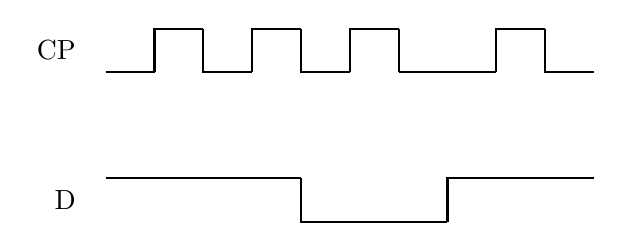
\begin{tikzpicture}[x=1cm, y=1cm, font=\normalsize, line width=0.8pt]
  \def\seg{0.62}   % 每段宽度（10 段）
  \def\hi{0.55}    % 高电平高度

  % CP 波形：0 1 0 1 0 1 0 0 1 0
  \begin{scope}[yshift=0cm]
    \node[anchor=east] at (-0.25,\hi/2) {CP};
    \draw (0,0) -- (\seg,0);                                    % 段1: 0
    \draw (\seg,0) -- (\seg,\hi) -- (2*\seg,\hi);                % 段2: 1
    \draw (2*\seg,\hi) -- (2*\seg,0) -- (3*\seg,0);              % 段3: 0
    \draw (3*\seg,0) -- (3*\seg,\hi) -- (4*\seg,\hi);            % 段4: 1
    \draw (4*\seg,\hi) -- (4*\seg,0) -- (5*\seg,0);              % 段5: 0
    \draw (5*\seg,0) -- (5*\seg,\hi) -- (6*\seg,\hi);            % 段6: 1
    \draw (6*\seg,\hi) -- (6*\seg,0);                            % 段7: 0
    \draw (6*\seg,0) -- (8*\seg,0);                              % 段8: 0
    \draw (8*\seg,0) -- (8*\seg,\hi) -- (9*\seg,\hi);            % 段9: 1
    \draw (9*\seg,\hi) -- (9*\seg,0) -- (10*\seg,0);             % 段10: 0
  \end{scope}

  % D 波形：1 1 1 1 0 0 0 1 1 1
  \begin{scope}[yshift=-1.9cm]
    \node[anchor=east] at (-0.25,\hi/2) {D};
    \draw (0,\hi) -- (4*\seg,\hi);                               % 段1-4: 1
    \draw (4*\seg,\hi) -- (4*\seg,0) -- (7*\seg,0);               % 段5-7: 0
    \draw (7*\seg,0) -- (7*\seg,\hi) -- (10*\seg,\hi);            % 段8-10: 1
  \end{scope}
\end{tikzpicture}
\end{document}
